% f2000_spring_jingwan_science_q22_parabola.tex — 2000 年·春季京皖卷·理科 第 22 题（抛物线 y²=4px 与动点 A、B、M）
%
% 【来源】`.work/phase4-b20/source/2000春季京皖理.pdf`
%   （SHA-256 37f07244497aa0a21be12d8a31eac78b61490f835f088719a5990463585a35ce），
%   第 2 页（印刷页 62）；qpdf --qdf 解包后对内容流逐路径解析。
% 【坐标口径】源 PDF 用户空间（原点左下、y 向上）。本图本地坐标
%   (x, y) = (x_page − 329.307, y_page − 687.581)，1 单位 = 1 TeX pt；
%   O 取两轴交点；x 轴 y_page ≡ 687.581，y 轴 x_page ≡ 329.307。
% 【元素计数】10 条绘制路径（x 轴／x 箭头／y 轴／y 箭头／AB／OA／OB／OM／抛物线上支／下支）＋ 6 个标签。
%   源内容流为 11 条：其中路径 6（直线 O→A）与路径 10（贝塞尔 O→A）几何重合，已合并。
% 【标签】位置取 pdftotext -bbox 文本中心换算（源中心逐条记在 \node 行末）；
%   本图各标签按源中心放置，无微调。
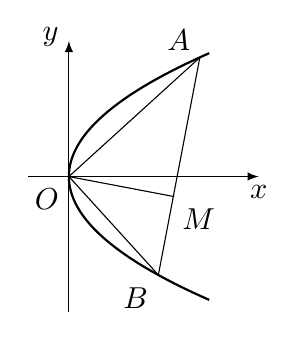
\begin{tikzpicture}[x=1pt, y=1pt,
    every node/.style={inner sep=0pt, font=\fontsize{10.5pt}{12.6pt}\selectfont}]
  \draw[line width=0.399pt] (-14.695,0) -- (64.989,0);
  \fill[line width=0.399pt] (68.576,0) .. controls (67.513,0.199) and (65.786,0.797) .. (64.591,1.494) -- (64.591,-1.494) .. controls (65.786,-0.797) and (67.513,-0.199) .. (68.576,0);
  \draw[line width=0.399pt] (0,-48.983) -- (0,45.396);
  \fill[line width=0.399pt] (0,48.983) .. controls (-0.199,47.92) and (-0.797,46.193) .. (-1.494,44.998) -- (1.494,44.998) .. controls (0.797,46.193) and (0.199,47.92) .. (0,48.983);
  % 三条割线。源内容流中 OB（路径 8）、OM（路径 9）以密集三次贝塞尔绘制，
  % 与直线最大偏差 0.0002 pt，此处按直线写出；O→A 另有路径 6（直线）与路径 10（贝塞尔）
  % 几何重合（偏差 < 0.01 pt），合并为一条。
  \draw[line width=0.399pt] (32.329,-35.562) -- (47.317,43.007);   % AB
  \draw[line width=0.399pt] (0,0) -- (47.317,43.007);              % OA
  \draw[line width=0.399pt] (0,0) -- (32.329,-35.562);             % OB
  \draw[line width=0.399pt] (0,0) -- (38.108,-7.269);              % OM
  % 抛物线 y^2 = 4px 的上、下两支（源路径 7 / 11，各 24 段三次贝塞尔）。
  % 拟合 x = 0.0255212 y^2（rms 0.0025 pt），即 4p = 39.177 pt。
  \draw[line width=0.797pt, domain=0:44.5724, samples=120, variable=\y]
    plot ({0.0255212*\y*\y}, \y);
  \draw[line width=0.797pt, domain=-44.5724:0, samples=120, variable=\y]
    plot ({0.0255212*\y*\y}, \y);

  \node[anchor=center] at (-6.647,50.369) {$y$};  % 源中心 (322.66,737.95)
  \node[anchor=center] at (39.683,49.329) {$A$};  % 源中心 (368.99,736.91)
  \node[anchor=center] at (68.573,-5.591) {$x$};  % 源中心 (397.88,681.99)
  \node[anchor=center] at (-7.997,-8.251) {$O$};  % 源中心 (321.31,679.33)
  \node[anchor=center] at (46.903,-15.521) {$M$};  % 源中心 (376.21,672.06)
  \node[anchor=center] at (24.123,-43.811) {$B$};  % 源中心 (353.43,643.77)
\end{tikzpicture}
%
% 【自验】
%   1) 探针编译：0 error、0 warning。
%   2) 600 dpi 双渲染差分量测标签净距：x 2.81、A 3.88、O 4.32、y 5.20、M 5.86、B 6.44 —— 最小 2.81 pt。
%   3) 线形：两轴与三条割线 0.399 pt；抛物线两支 0.797 pt，与源 w、d 值一致（全为实线）。
%   4) 抛物线拟合残差 rms 0.0025 pt；A、B 落在抛物线上（偏差 0.1 pt 内），OA⊥OB 斜率积 −1.000。
